\chapter{Mensuration}
Real application of the book starts here. Through this chapter, students will be able to learn the following things:
\begin{itemize}
	\item Determining the area of polygonal region by applying the laws of area of triangle and quadrilateral and solve allied problems.
	\item Determining the area, circumference and length of chord of a circle.
	\item Determining the area and the volume of solid rectangles, cubes and cylinders and solving the problems related to it.
	\item Determining the area and the volume of uniform solids.
\end{itemize}

\section{Area of triangles}
We learned about triangle and it's different shapes with respect to sides angles and other parameters. We also learned the formula of area of a triangle which is, 
\begin{equation}
	\label{one}
	A= \frac{1}{2}\times base \times height
\end{equation}
But the problem is that this formula has limitations. The triangles which do not contain height can't be found the area by this formula. In this case, we only have height in right angled triangle. Otherwise, we have to find the height explicitly and put it into \autoref{one}. Now we simplify this formula considering above discussion for various types of triangles:

\subsection{Right angled triangle}
\begin{wrapfigure}{r}{.35\textwidth}
	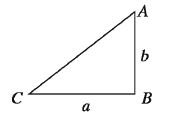
\includegraphics[width=1.9in]{pics/rat}
\end{wrapfigure}
Since the right angled triangle has height, we can assume the \autoref{one} as the formula of area. For a triangle $ABC$ with height $AB=b$ \& base $BC=a$, we will have the area of $\triangle ABC$,\\

\begin{equation}
	\label{e1}
	A= \frac{1}{2}\times BC \times AB = \frac{1}{2}ab
\end{equation}

\subsection{Two sides with common adjacent angle}
\begin{wrapfigure}{r}{.35\textwidth}
	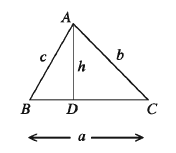
\includegraphics[width=1.9in]{pics/sas}
\end{wrapfigure}
We can find the height of triangle if angle is given. And then we put the height in \autoref{one}. The process is as follows:

$\frac{AD}{AB} = \frac{h}{c} = sinB$\\
$\implies h= c\times sinB$\\
$\implies \frac{1}{2}\times BC \times AD=a\times c\times sinB$\\
and similarly,\\ $a\times c\times sinB = a\times b\times sinC = b\times c\times sinA$
Then the area is,
\begin{equation}
\label{e2}
A= a\times c\times sinB = a\times b\times sinC = b\times c\times sinA
\end{equation}


\subsection{Three sides}
\begin{wrapfigure}{r}{.35\textwidth}
	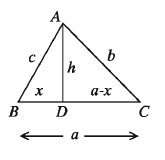
\includegraphics[width=1.9in]{pics/sss}
\end{wrapfigure}
We can use the formula of Pythagoras to find the area like\\

$AD^2=AB^2-BD^2$ and\\ $AD^2=AC^2-CD^2$ \\ $\therefore AB^2-BD^2 = AC^2-CD^2 $\\
$
\implies c^2-x^2=b^2-(a-x)^2\\
\implies c^2-x^2=b^2-a^2-x^2+2ax\\
\implies 2ax=c^2-b^2+a^2\\
\therefore x=\frac{c^2+a^2-b^2}{2a}\\[2ex]
$
Moreover,
\begin{align*}
AD^2&=c^2-x^2\\
	&=c^2-(\frac{c^2+a^2-b^2}{2a})^2\\
	&=\left(c+(\frac{c^2+a^2-b^2}{2a})\right)\left(c-(\frac{c^2+a^2-b^2}{2a})\right)\\
	&=\left(\frac{2ac+c^2+a^2-b^2}{2a}\right)\cdot \left(\frac{2ac-c^2-a^2+b^2}{2a}\right)\\
	&=\frac{\{(c+a)^2-b^2\}\cdot\{b^2-(c-a)^2\}}{4a^2}\\
	&=\frac{(a+b+c)(c+a-b)(b+c-a)(b-c+a)}{4a^2}\\
	&=\frac{(a+b+c)(a+b+c-2b)(a+b+c-2a)(a+b+c-2c)}{4a^2}\\
	&=\frac{2s(2s-2b)(2s-2a)(2s-2c)}{4a^2}\hspace*{2cm} [Taking\; 2s=a+b+c]\\
	&=\frac{4s(s-a)(s-b)(s-c)}{a^2}\\
\end{align*}
$ \therefore AD=\frac{2}{a}\sqrt{s(s-a)(s-b)(s-c)}\\[1ex]$
$\therefore$ Area of $\triangle ABC=\frac{1}{2}\cdot a\cdot \frac{2}{a}\sqrt{s(s-a)(s-b)(s-c)}$

\begin{equation}\label{e3}
	\therefore A=\sqrt{s(s-a)(s-b)(s-c)}
\end{equation}
$ where \;s=\frac{a+b+c}{2}$, namely half of the perimeter.


\subsection{Equilateral triangle}
\begin{wrapfigure}{r}{.35\textwidth}
	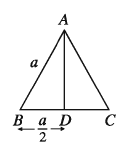
\includegraphics[width=1.9in]{pics/elt}
\end{wrapfigure}
Since this type of triangle has the same length of every side, we take $AB=BC=AC=a$
Then $AD^2=AB^2-BD^2=a^2-(a/2)^2=3a^2/4\\$ $[ since\; AD$ is median and $BD=CD=\frac{a}{2} ]\\$
$\therefore AD=\frac{\sqrt{3}a}{2}$\\

Then area of $\triangle ABC$,
\begin{equation}\label{e4}
A= \frac{1}{2}\cdot a\cdot \frac{\sqrt{3}a}{2}=\frac{\sqrt{3}a^2}{4}
\end{equation}


\subsection{Isosceles triangle}
\begin{wrapfigure}{r}{.35\textwidth}
	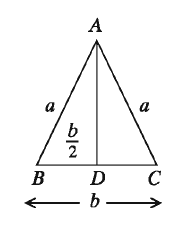
\includegraphics[width=1.9in]{pics/ist}
\end{wrapfigure}
This type of triangles has two same sides, namely $AB=AC=a,\; BC=b$ and $BD=b/2$. Here we again attempt to find the height $AD$ with Pythagoras' formula.\\

Then $AD^2=AB^2-BD^2\\
=a^2-(\frac{b}{2})^2\\
=a^2-\frac{b^2}{4}\\
=\frac{4a^2-b^2}{4}\\
\therefore AD=\frac{\sqrt{4a^2-b^2}}{2}\\$

Hence Area of $\triangle ABC= \frac{1}{2}\cdot b\cdot \frac{\sqrt{4a^2-b^2}}{2}$
\begin{equation}\label{e5}
	\therefore A=\frac{b}{4}\sqrt{4a^2-b^2}
\end{equation}



\begin{wrapfigure}{r}{.35\textwidth}
	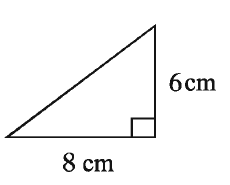
\includegraphics[width=1.9in]{pics/e1}
\end{wrapfigure}
\begin{exmp}
Let the lengths of two sides of a right triangle, adjacent to right angle are both 6 cm  respectively. Lets find the area using the formulas we've just derived.
\end{exmp}
\textbf{Sol$^n$:}\\ 
Here Let $a=6,\; b=6\; \angle C=90\degree\\$


Using \autoref{e1}: $A=\frac{1}{2}ab=\frac{6\times6}{2}=18\;cm^2\\$


Using \autoref{e2}: $A=\frac{1}{2}ab\;\sin C=\frac{1}{2}\times6\times6\times \sin 90\degree=18\;cm^2$


Using \autoref{e3}: 
First we have to find the $3^{rd}$ side of the triangle using Pythagoras formula, that is,\\
$c^2=a^2+b^2\\
\implies c=\sqrt{a^2+b^2}\;cm\\
\implies c=\sqrt{6^2+6^2}\;cm\\
\implies c=6\sqrt{2}\;cm$\\[1ex]
Again $s=\frac{1}{2}(a+b+c)=\frac{6+6+6\sqrt{2}}{2}=6+3\sqrt{2}\;cm\\$
Then the area of the triangle,\\$A=\displaystyle \sqrt{s(s-a)(s-b)(s-c)}\; sq\;unit$
\\$\implies A=\displaystyle \sqrt{(6+3\sqrt{2})\cdot(6+3\sqrt{2}-6)\cdot(6+3\sqrt{2}-6)\cdot(6+3\sqrt{2}-6\sqrt{2})}\;cm^2$
\\$\implies A=\displaystyle \sqrt{(6+3\sqrt{2})\times 3\sqrt{2}\times 3\sqrt{2}\times (6-3\sqrt{2})}\;cm^2$
\\$\implies A=\displaystyle \sqrt{(3\sqrt{2})^2\times (6^2-(3\sqrt{2})^2)}\;cm^2$
\\$\implies A=\displaystyle \sqrt{18^2}\;cm^2$
\\$\implies A=\displaystyle 18 \;cm^2$


Using \autoref{e5}:
Here we can use the formula to find the area, that is,\\

$\displaystyle A=\frac{c}{4}\sqrt{4a^2-c^2}
\\=\frac{6\sqrt{2}}{4}\cdot \sqrt{4\times 6^2-(6\sqrt{2})^2}
\\=\frac{6\sqrt{2}}{4}\cdot \sqrt{6^2\times2}
\\=\frac{6\sqrt{2}}{4}\cdot 6\times\sqrt{2}
\\=\frac{6\times6\times2}{4}
\\=18\;cm^2$


Thus we showed all the formulas to find the area of a triangle except for \autoref{e4} since that triangle is not equilateral. Let us suppose for instance that all three sides of the triangle is of 6 cm. Then we can find the area of the triangle using \autoref{e4}, that is,\\

$\displaystyle A=\frac{\sqrt{3}}{4}\cdot 6^2=9\sqrt{3}\;cm^2$


\begin{wrapfigure}{r}{.35\textwidth}
	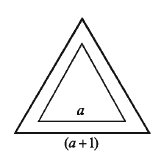
\includegraphics[width=1.9in]{pics/e2}
\end{wrapfigure}
\begin{exmp}
	The area of an equilateral triangle increases by $3\sqrt{3}$ sq. meter when the length of each side increases by 1 meter. Find the length of the side of the triangle
\end{exmp}


\textbf{Solution:\\}Let, the length of each side of the equilateral triangle is a meter.\\
$\therefore$ It's area= $\frac{\sqrt{3}}{4}a^2$ sq. meter.\\
The area of the triangle when the length of each side increases by 1 meter= $\frac{\sqrt{3}}{4}(a+1)^2$ sq. meter.\\

According to question, $$\ds\frac{\sqrt{3}}{4}(a+1)^2-\frac{\sqrt{3}}{4}(a+1)^2=3\sqrt{3}$$
$\implies (a+1)^2-a^2=12\\$
$\implies (a+1+a)(a+1-a)=12\\$
$\implies 2a+1=12\\$
$\implies 2a=12-1=11\\$
$\implies a=5.5\\$
Therefore, the required length is 5.5 meter.





\begin{exmp}
	From a certain place two roads run in two directions making an angle of $120\degree$ From that place the person move in two directions with the speed of 10kmh and 8kmh respectively. What will be the direct distance between them after 5 hours?
\end{exmp}

\textbf{Solution:\\}Let two men start from $A$ with velocities 10kmh and 8kmh respectively and reach $B$ and $C$ after 5 hours. Then after 5 hours, the direct distance between them is $BC$. From $C$ perpendicular $CD$ is drawn on $BA$ produced.\\
\begin{wrapfigure}{r}{.35\textwidth}
	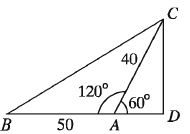
\includegraphics[width=1.9in]{pics/e3}
\end{wrapfigure}
$\therefore AB=5\times 10km=50km, \\AC=5\times 8km = 40 km \;\& \;\angle BAC=120\degree\\$
$\therefore DAC=180 \degree-120\degree=60\degree\\$
$\triangle ACD$ is right angled.\\
$\therefore \ds \frac{DC}{AC}=\sin 60\degree\\$
$\implies \ds DC=AC\sin 60\degree\\= 40\times \frac{\sqrt{3}}{2}=20\sqrt{3}\\$


Again $ \ds \frac{AD}{AC}=\cos 60\degree\\$
$\implies \ds AD=AC\cos 60\degree= 40\times \frac{1}{2}=20\\$

Again, from right angled triangle $BCD$ we get,\\
$BC^2=BD^2+CD^2=(BA+AD)^2+CD^2\\=(50+20)^2+(20\sqrt{3})^2=4900+1200=6100\\[1ex]\therefore BC=78.1\\$
Then the distance is=78.1 km.

\begin{exmp}
	Consider the diagram given and-
	\begin{enumerate}
		\item Find the length of the side $BC$
		\item Find the value of $BD$?
		\item Find the ratio of areas of the triangles $\triangle ABD$ and $\triangle BCD$.
	\end{enumerate}
\end{exmp}
\textbf{Solution:}
	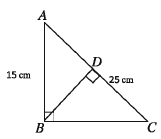
\includegraphics[width=1.9in]{pics/e4}

\begin{enumerate}
	\item $AB=15,\;AC=25\\ \therefore BC=\sqrt{AC^2-AB^2}=\sqrt{25^2-15^2}=\sqrt{400}=20$
	\item Area of triangle $\triangle ABC= \frac{1}{2}BC\cdot AB=\frac{1}{2}AC\cdot BD\\
	\implies 25\times BD=20\times 15\\ \therefore BD=12\\$
	\item From the right angled triangle $\triangle ABD$ we get\\
	$AD^2+BD^2=AB^2\\
	\implies AD^2+12^2=15^2\\
	\implies AD^2=225-144=81\\
	\implies AD=9\; \& \; CD=AC-AD=25-9=16\\$
	So, ratio of areas of $\triangle ABD$ and $\triangle BCD$ is:\\
	
	$\ds \frac{\triangle ABD} {\triangle BCD}=\frac{\ds\frac{1}{2}BD\cdot AD}{\ds\frac{1}{2}BD\cdot CD}=\frac{9}{16}\\[1em]
	\therefore\triangle ABD : \triangle BCD=9 : 16\\[3ex]$ 
	
\end{enumerate}
\textbf{\Large Exercise 16.1\\[2ex]}
\begin{enumerate}
	\item The hypotenuse of a right angled triangle is 25 m. If one of its sides is $\frac{3}{4}$ of the other, find the length of the two sides.
	\item A ladder with length 20 m stands vertically against a wall. How much further should the lower end of the ladder be moved so that its upper end descends 4 meter?
	\item The perimeter of an isosceles triangle is 16 m. If the length of equal sides is $\frac{5}{6}$ of base, find the area of the triangle.
	\item The lengths of the two sides of a triangle are 35 cm, 27cm and perimeter is 84 cm. Find the area of the triangle.
	\item When the length of each side of an equilateral triangle is increased by 2 m, its area is increased by $6\sqrt{3}$ square meter. Find the length of side of the triangle.
	\item The lengths of two sides of a triangle are 26 m, 28 m respectively and its area is 182 $m^2$. Find the angle between the two sides.
	\item The length if equal sides of an isosceles triangle is 10 m, and 48 $m^2$. Find the length of the base.
	\item Two roads run from a certain place with an angle of $135\degree$ in two directions. Two persons move from that place in two directions with the speed of 7 kmh and 5 kmh respectively. What will be the direct distance between them after 4 hours?
	\item If the lengths of the perpendiculars from a point interior of an equilateral triangle to three sides are 6 cm, 7 cm and 8 cm respectively; Find the length of sides of the triangle and the area of the triangular region.
	\item The perpendicular of a right angled triangle is 6 cm less than $\frac{11}{12}$ times of the base, and the hypotenuse is 3 cm less than $\frac{4}{3}$ times of the base.
	\begin{enumerate}
		\item Let the base be $x$. Express the area of the triangle in terms of $x$.
		\item Find the length of the base
		\item If the length of the base of the triangle is 12 cm, find the area of the equilateral triangle having the perimeter equals to it.
	\end{enumerate}
\end{enumerate}







































